\documentclass[a4paper, 11pt, titlepage]{jsarticle}
\usepackage[dvipdfmx]{graphicx}
\usepackage{listings}
\usepackage{amsmath}
\usepackage{url}
\usepackage{float}
\usepackage{multirow}


\title{知能情報総合実験(データマイニング班)\\機械学習で地域予測をしてみる}
\author{235728D 勇夢亜
 235730F  塩田翼 \\
235716A 仲宗根朝飛
 235727F 兼島響太朗  \\
}
\date{提出日:2025年7月31日}
\begin{document}
\maketitle
\tableofcontents


\abstract{本レポートでは、風景画像からの地域予測タスクにおける機械学習モデルの有効性を検証した。特に、データセットの画像数に偏りがあるという課題に対し、データサンプリング戦略の調整や損失関数へのクラス重み付け導入といった複数のアプローチを試みた。畳み込みニューラルネットワーク(CNN)の一種であるDenseNetをモデルとして採用し、学習率や画像サイズなどのハイパーパラメータ調整を行った。実験の結果、最適なハイパーパラメータ設定(学習率0.0001、画像サイズ224)とデータ処理戦略により、最終的に80.78\%の全体正答率を達成した。混同行列の分析からは、地理的に近い地域間での誤分類が多い傾向が確認された。}

\section{はじめに}

\subsection{テーマ:場所推測とは}

本グループでは、風景画像からの位置情報の推定を対象問題として設定した。これは、GPSなどの位置情報が取得できない状況や、既存の地図情報が不十分な地域において、画像から得られる視覚的な手がかりをもとに場所を推定する技術の構築を目指すものである。今回の実験では、風景画像を用いて撮影地点の国または地域を予測するタスクに取り組む。
この問題設定の背景には、「ジオゲッサー(GeoGuessr)」というゲームの存在がある\cite{geoguessr}。ユーザーは提示された風景画像をもとに、世界地図上で撮影場所を推測する。このタスクでは、自然風景や人工物、道路標識、建築様式、植生など、画像中の視覚的な特徴から地理的な手がかりを抽出する必要があり、機械学習による画像認識技術や地理情報処理の実践的応用が期待される。
本研究の目的は、画像認識モデルを用いて与えられた画像の撮影地点を高精度で推定することである。特に、モデルの構築にあたっては、畳み込みニューラルネットワーク(CNN)などの画像分類モデルを活用し、画像に含まれる特徴量と地理情報の関係性を学習させる。また、予測精度の向上を図るために、誤分類された事例についてその原因を分析し、地域ごとの特徴の類似性やモデルの過学習傾向を考慮した改良を行う方針である。
この技術は、観光支援や災害時の被災地の迅速な特定、衛星画像やドローン映像の解析など、さまざまな場面での応用が期待される。今回の実験では、まず国単位での位置推定において70\%以上の分類精度を目標とし、その達成に向けてモデル設計とデータ処理手法の最適化を進めていく。

\section{実験方法}

\subsection{データセット構築}
本実験では、Kaggleにて公開されている国ごとの風景画像データセット「GeoLocation - Geoguessr Images(50K)」\cite{geolocation}をダウンロードし、利用した。このデータセットは、約50,000枚の画像で構成されており、各国の画像枚数には大きく偏りがあった。

本研究では、国ごとのデータセットを以下の8つの地域に分類し、地域予測のタスクに取り組んだ。
\begin{itemize}
    \item アジア
    \item 日本
    \item 中東
    \item 北アメリカ
    \item 南アメリカ
    \item ヨーロッパ
    \item アフリカ
    \item オセアニア
\end{itemize}
この分類は、国単位で学習を行った場合に、国ごとの画像枚数の不均衡が精度に直接的に影響を与えるという懸念から行われた。実際に、類似のデータセットを用いた先行研究\cite{kaggle_geoguesser}では、画像数の少ない国の精度が低くなる傾向が報告されている。そこで、地理的に近い国をグループ化することで、各クラスのデータ数をある程度均一化し、モデルがより汎化された特徴を学習できるようにすることを目的とした。

当初、データセット内の地域ごとの画像数に顕著な偏りがあることが判明した。特に、データ数の多い地域への予測が偏り、データ数の少ない地域(例:中東)ではモデルが十分に学習できず、予測精度が低いという問題が発生した。この偏りの影響を評価するため、まず約50,000枚の全データを用いて実験を行った。

この偏りを解消し、モデルの汎化性能を向上させるため、複数のアプローチを試みた。

まず、データ量の減少による情報損失が懸念されたものの、全ての地域から800枚のデータを抽出して使用する構成で実験を行った。

次に、データ量の減少を抑えつつ、少数クラスのデータ量を確保することを目的として、中東地域からは800枚、その他の地域からはそれぞれ2000枚の画像をランダムに抽出して使用する構成で実験を行った。

最終的に、これらのサンプリングによるデータ量減少の懸念を考慮し、約50,000枚の全データを使用しつつ、学習時にクラスの不均衡を是正するために損失関数に重み付けを施す手法も採用した。損失関数の重みは、各クラスのサンプル数の逆数に応じて算出された。具体的には、クラス$c$の重み$w_c$を、$w_c = N / (C \times N_c)$ のように設定した。ここで、$N$は全サンプル数、$C$はクラス数、$N_c$はクラス$c$のサンプル数である。これにより、データが少ない地域の影響を学習時に大きく反映させ、偏りを軽減することを目指した。

\subsection{モデル選定}
本実験では、畳み込みニューラルネットワーク(CNN)の一種であるDenseNetを採用した\cite{densenet_article}。DenseNetは、各層がそれ以前のすべての層からの出力を入力として受け取る「密な接続」を持つことが特徴であり、これにより特徴の再利用が促進され、勾配消失問題が緩和される。画像認識タスクにおいて高い性能を示すことが知られており、特に複雑な画像データからの特徴抽出に優れているため、風景画像からの地域予測という本タスクに適していると判断した。

\subsection{パラメータ調整方法}
本実験では、モデルの性能を最大化するために、学習率 (Learning Rate)、画像サイズ (Image Size) の主要なハイパーパラメータについて調整を行った。エポック数 (Epochs) は30で実行し、学習曲線(図\ref{fig:epochs_training_loss_accuracy})から20エポックを超えたあたりで安定し始めたことを確認した。バッチサイズ (Batch Size) は16に固定し、これはSimpleCNNの実験で決定された値を踏襲した(図\ref{fig:batch_size})。これらのパラメータは、\lstinline{hyperparameter_tuning.py}スクリプトを用いて、複数の候補値を試行し、それぞれの組み合わせにおけるモデルの精度と学習挙動を比較検討することで最適な値を決定した。特に、学習率と画像サイズについては、異なる値での実験結果を比較し、最も高い精度が得られる組み合わせを採用した。

\begin{figure}[H]
  \centering
  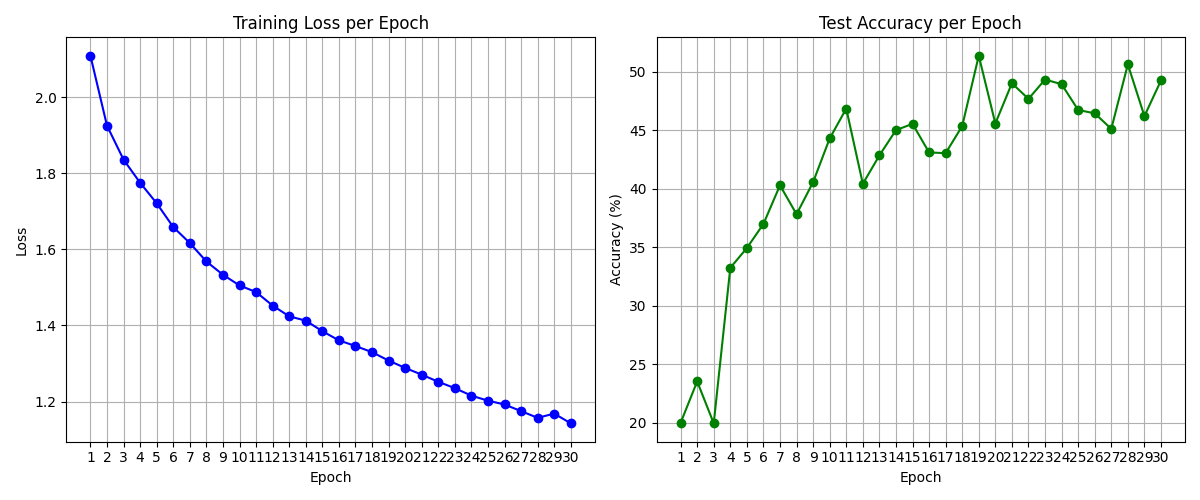
\includegraphics[width=0.8\linewidth]{use/epochs_training_loss_accuracy.png}
  \caption{学習曲線 (バッチサイズ16): エポック数に対するトレーニングロスと精度を示す。}
  \label{fig:epochs_training_loss_accuracy}
\end{figure}

\begin{figure}[H]
  \centering
  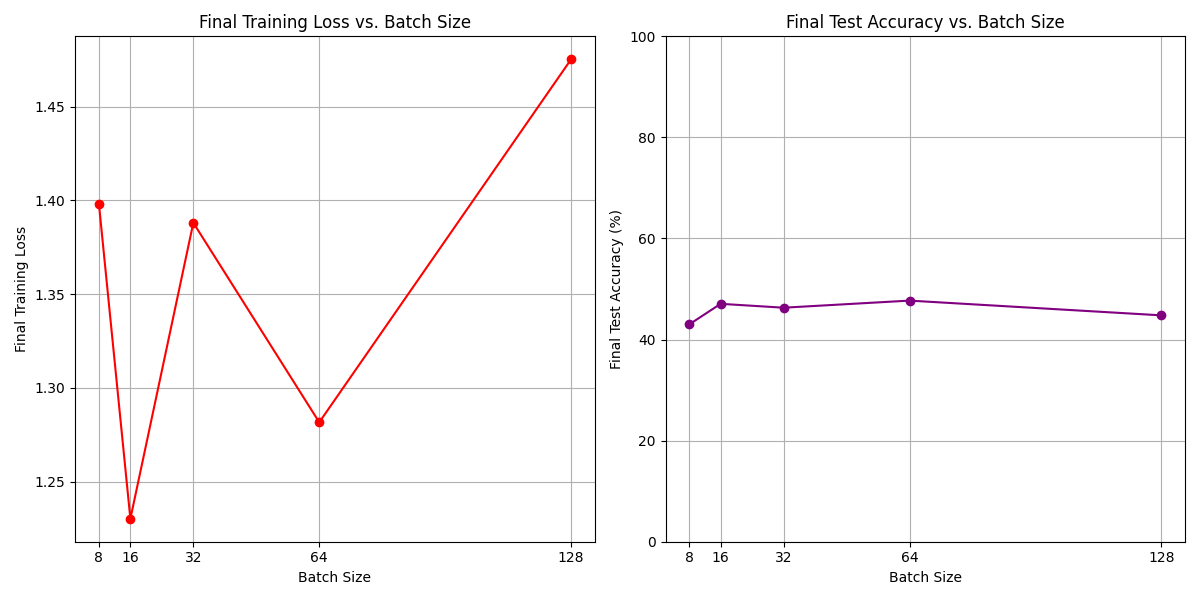
\includegraphics[width=0.8\linewidth]{use/batch.png}
  \caption{バッチサイズと学習曲線: バッチサイズ16における学習曲線を示す。}
  \label{fig:batch_size}
\end{figure}


\section{実験結果}
本実験では、DenseNetを用いて風景画像からの地域予測を行った。様々なデータセット構成とハイパーパラメータ設定で実験を行い、その結果を以下に示す。

\subsection{DenseNetの全体精度}
本実験では、DenseNetを用いて風景画像からの地域予測を行った。様々なデータセット構成とハイパーパラメータ設定で実験を行い、その結果を以下に示す。

ハイパーパラメータ調整の結果、学習率0.0001、画像サイズ224の組み合わせで最も高い精度が得られた。この設定におけるDenseNetのテストデータに対する全体での正解率は80.78\%であった。

\subsection{混同行列}
本実験で得られた混同行列を以下に示す(図\ref{fig:conf_matrix_all_data}~\ref{fig:conf_matrix_optimal_param})。これらの混同行列からは、データセットの構成や重み付けの有無、ハイパーパラメータの違いがモデルの予測性能に与える影響が明確に確認された。特に、地理的に近い、あるいは景観が類似している地域間での誤分類が多く見られた。

\begin{figure}[H]
  \centering
  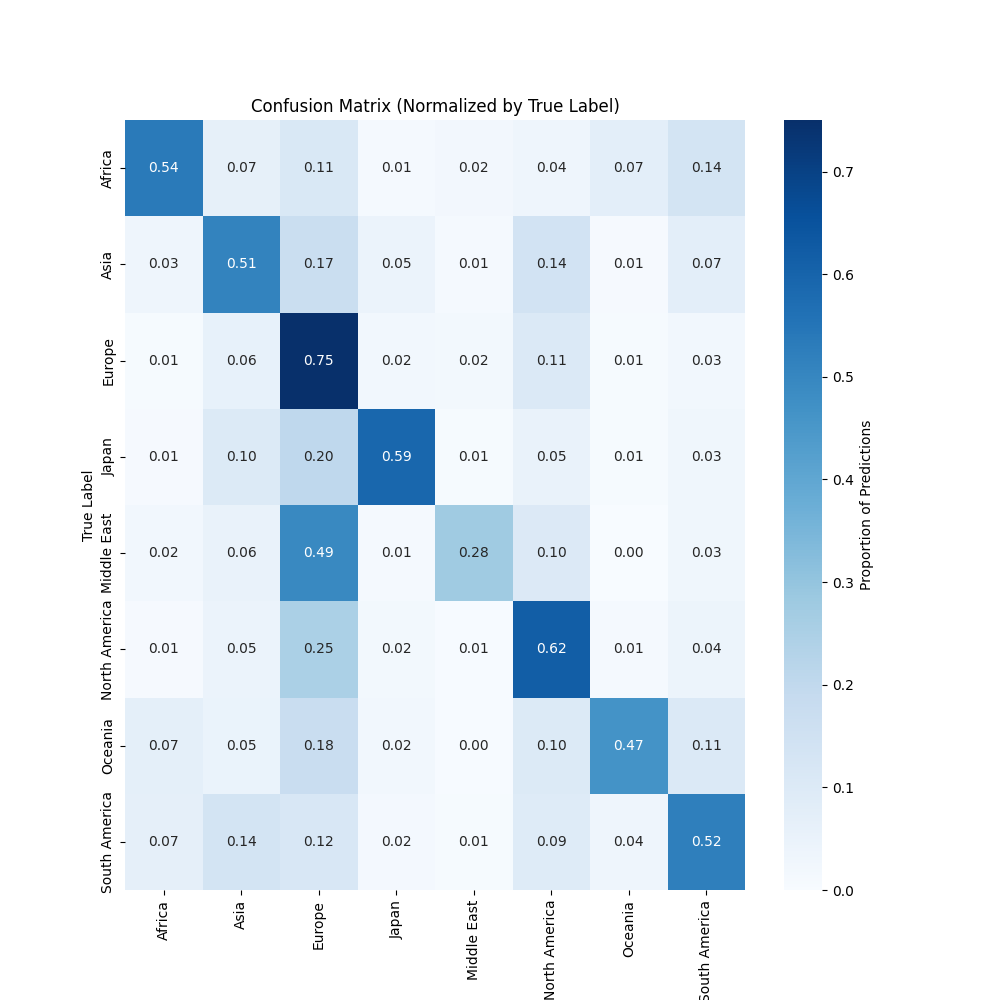
\includegraphics[width=0.8\linewidth]{use/confusion_matrix_heatmap.png}
  \caption{DenseNetの混同行列 (全データ使用、初期実験): 初期実験で約50,000枚の全データを用いた場合の混同行列。この設定での全体精度は 63.14\%であった。データ数の多い地域(例:ヨーロッパ、北アメリカ)への予測偏りが顕著に見られ、少数クラスの予測精度が低いことが確認された。}
  \label{fig:conf_matrix_all_data}
\end{figure}

\begin{figure}[H]
  \centering
  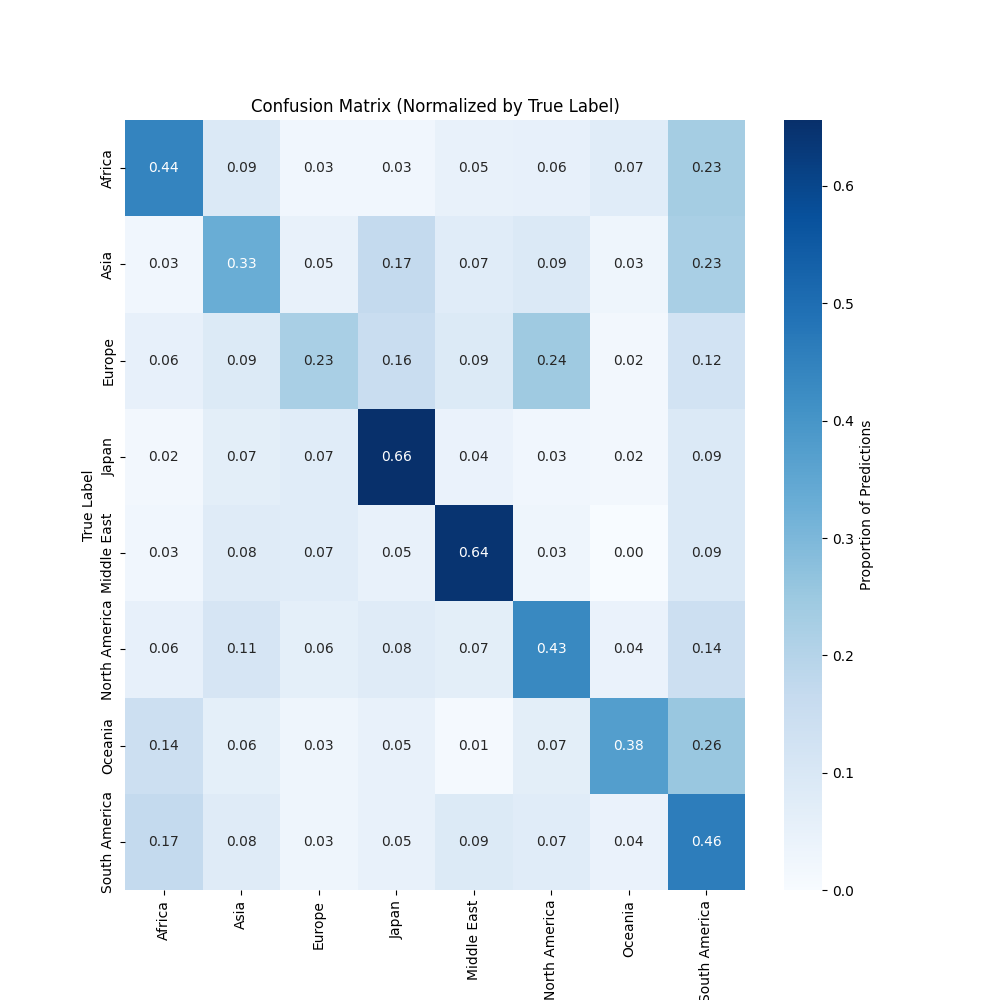
\includegraphics[width=0.8\linewidth]{use/densenet_all_800_matrix_heatmap.png}
  \caption{DenseNetの混同行列 (全地域800枚サンプリング): 全ての地域から800枚のデータを抽出して学習した場合の混同行列。この設定での全体精度は 44.63\%であった。データ量の減少による情報損失が予測性能に与える影響が示唆される。この設定では、特にアフリカやアジアといった地域で予測精度が低下する傾向が見られた。}
  \label{fig:conf_matrix_all_800}
\end{figure}

\begin{figure}[H]
  \centering
  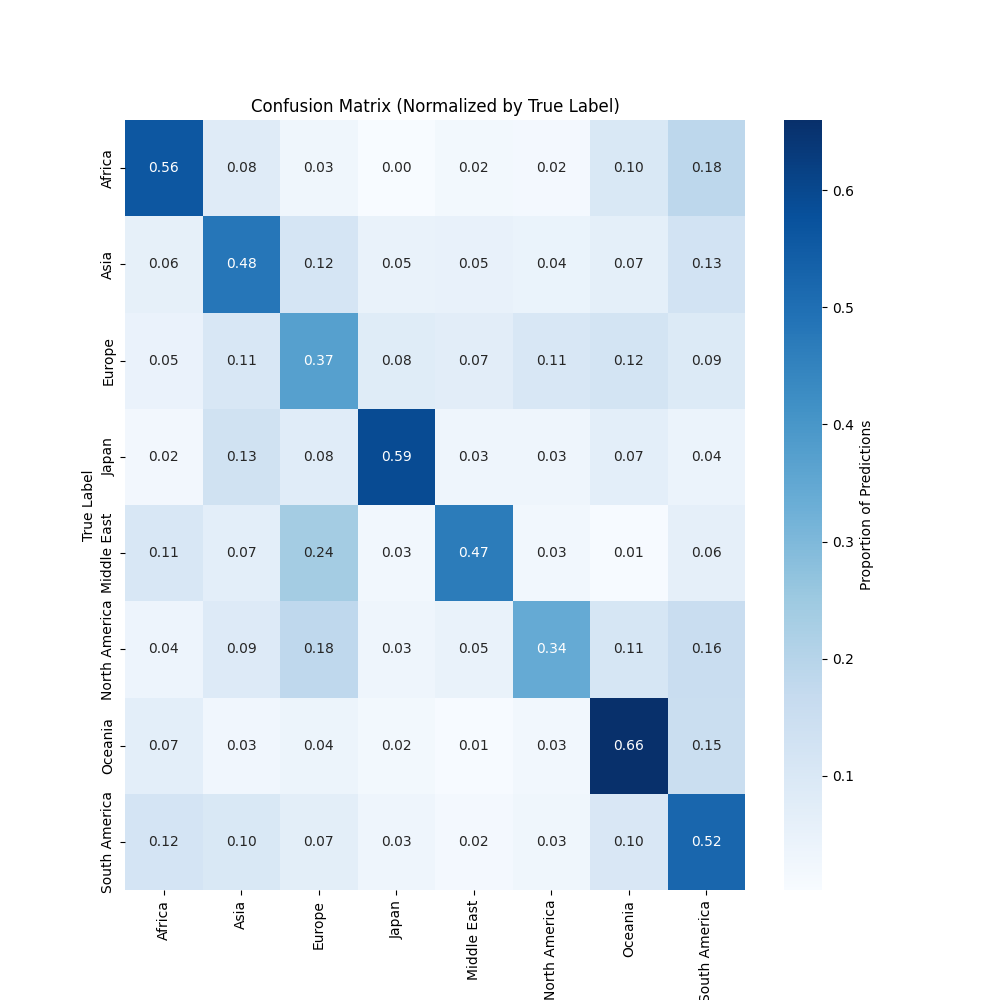
\includegraphics[width=0.8\linewidth]{use/densenet_adjusted_800_2000_total_confusion_matrix_heatmap.png}
  \caption{DenseNetの混同行列 (中東800枚、他2000枚サンプリング): データセットの全体的な予測性能向上を目的として、中東地域を800枚、その他の地域を2000枚に調整したデータセットを用いた場合の混同行列。この設定での全体精度は 49.22\%であった。全ての地域から800枚をサンプリングした場合と比較して、中東の自己予測精度は低下したものの、アフリカ、アジア、ヨーロッパ、オセアニア、南アメリカといった他の地域の予測精度が向上したことで、全体としての予測性能が改善された。}
  \label{fig:conf_matrix_adjusted_data}
\end{figure}

\begin{figure}[H]
  \centering
  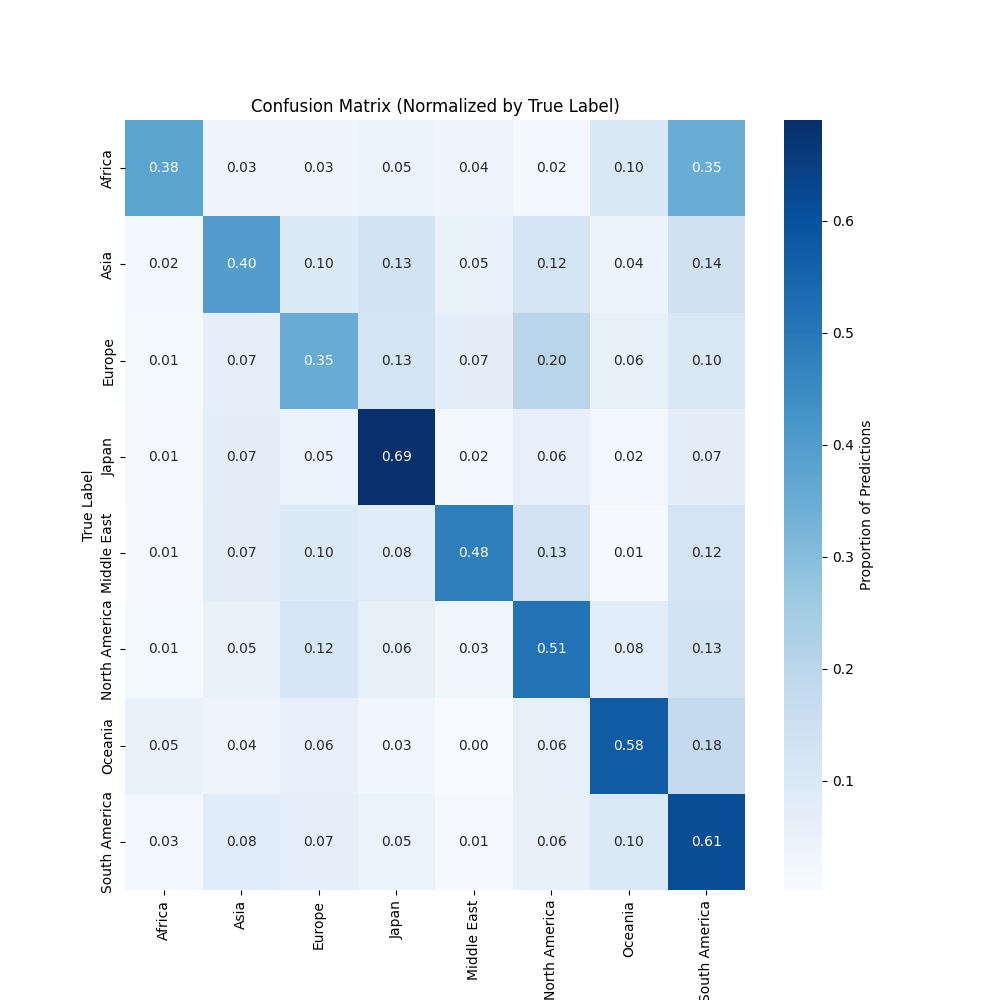
\includegraphics[width=0.8\linewidth]{use/confusion_balanced_matrix_heatmap.png}
  \caption{DenseNetの混同行列 (重み付けあり、全データ): クラス不均衡への対策として、損失関数にクラスごとの重み付けを導入して学習した場合の混同行列。この設定での全体精度は 46.34\%であった。重み付けなしの初期実験と比較して全体精度は低下したものの、少数クラスの予測精度が改善され、各クラスの予測がより均等になる傾向が見られた。}
  \label{fig:conf_matrix_balanced}
\end{figure}

\begin{figure}[H]
  \centering
  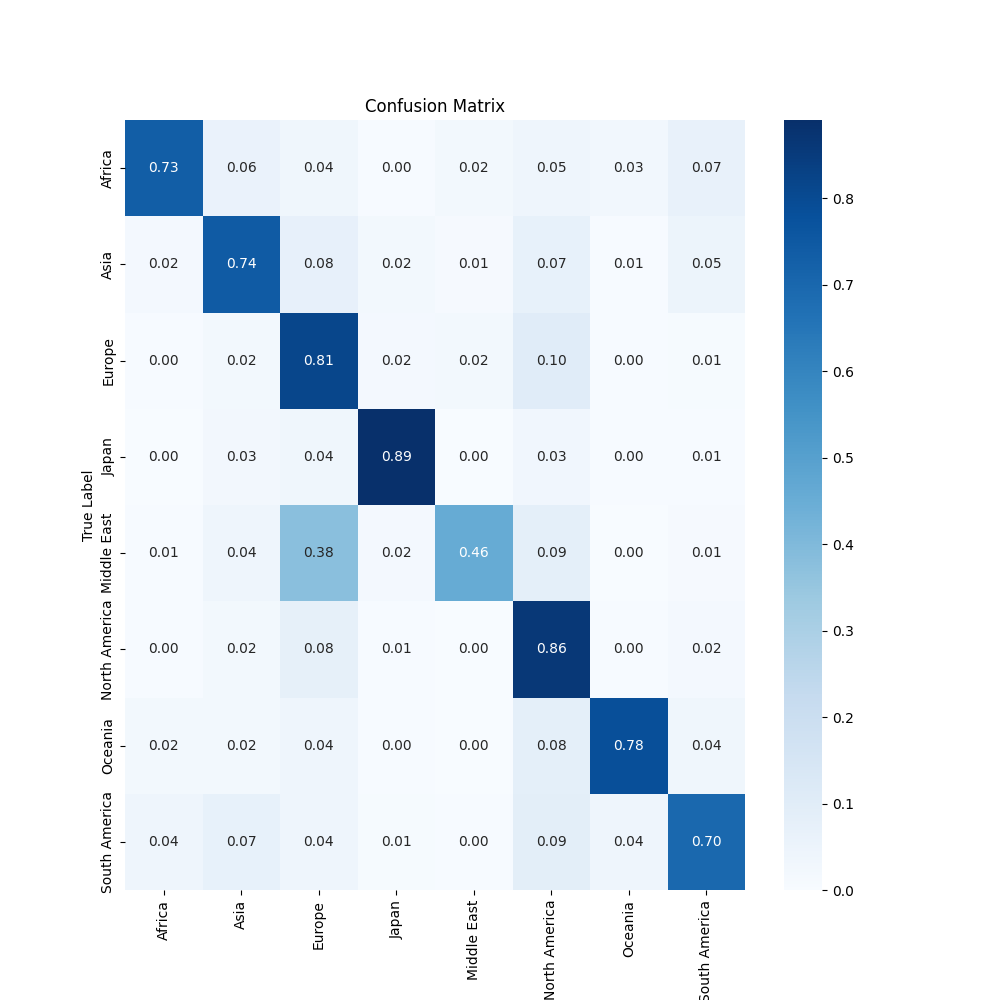
\includegraphics[width=0.8\linewidth]{use/lr_0.0001_size_224_confusion_matrix.png}
  \caption{DenseNetの混同行列 (最適パラメータでの結果): ハイパーパラメータを最適化した最終的なモデルの混同行列。学習率0.0001、画像サイズ224の組み合わせで学習されたモデルの結果であり、対角成分の数値が高く、全体的な予測精度が向上していることが示唆される。}
  \label{fig:conf_matrix_optimal_param}
\end{figure}

\subsubsection{ハイパーパラメータ調整結果}
以下に、ハイパーパラメータ調整の結果を示す(表\ref{tab:hyperparameter_tuning})。
\begin{table}[H]
  \centering
  \caption{ハイパーパラメータ調整結果}
  \label{tab:hyperparameter_tuning}
  \begin{tabular}{|c|c|c|c|c|}
    \hline
    \multicolumn{2}{|c|}{} & \multicolumn{3}{c|}{Image Size} \\
    \cline{3-5}
    \multicolumn{2}{|c|}{} & 64 & 128 & 224 \\
    \hline
    \multirow{3}{*}{Learning Rate} & 0.01 & 37.86\% & 41.48\% & 41.30\% \\
    \cline{2-5}
    & 0.001 & 48.98\% & 56.75\% & 51.34\% \\
    \cline{2-5}
    & 0.0001 & 65.68\% & 74.56\% & 80.78\% \\
    \hline
  \end{tabular}
\end{table}



\section{考察}各混同行列の分析から、データセットのサンプリング戦略や重み付けの有無がモデルの予測挙動に与える影響が明確に見て取れる。初期実験で約50,000枚の全データを用いた混同行列(図\ref{fig:conf_matrix_all_data}、全体正答率63.14\%)は、データ数の多い地域への予測偏りが顕著であった。全地域から800枚のデータをサンプリングした場合(図\ref{fig:conf_matrix_all_800}、全体正答率44.63\%)は、データ量の減少による情報損失が予測性能に影響することが示唆された。これに対し、中東地域を800枚、その他の地域を2000枚に調整したデータセット(図\ref{fig:conf_matrix_adjusted_data}、全体正答率49.22\%)では、中東の自己予測精度は低下したものの、アフリカ、アジア、ヨーロッパ、オセアニア、南アメリカといった他の地域の予測精度が向上したことで、全体としての予測性能が改善された。

クラス不均衡への対策として損失関数にクラスごとの重み付けを導入した全データでの実験(図\ref{fig:conf_matrix_balanced}、全体正答率46.34\%)では、重み付けなしの初期実験と比較して全体正答率は低下した。しかし、これはデータ数の多いクラスへの予測偏りを抑制し、データ数の少ないクラスの予測精度を向上させることで、各クラスの予測精度をより均等にすることを意図した結果である。実際、重み付けなしの初期実験では予測が特定のクラスに集中する傾向が見られたが、重み付けを導入することで、各クラスへの予測がより分散され、バランスの取れた予測が可能になった。この結果は、重み付けによるクラス不均衡対策が、全体の精度を犠牲にしてでも、各クラスの予測バランスを改善する効果を持つことを示唆している。

最終的に、最適パラメータで学習したモデルの混同行列(図\ref{fig:conf_matrix_optimal_param}、全体正答率80.78%)では、対角成分の数値が高く、全体的な予測精度が大幅に向上していることが示唆される。データ数の少ない中東地域に対しては、データサンプリング戦略の調整や、DenseNetにおけるクラス重み付けの導入といった対策を講じた。これらの対策により、モデルの汎化性能は向上したが、依然として特定の地域間での誤分類が見られる。特に、クラス重み付けを導入しても、絶対的なデータ数が少ないクラスでは学習できる特徴の多様性に限界があり、これが中東地域の正解率が伸び悩んだ一因と考えられる。

依然として特定の地域間での誤分類が見られることから、地域間の景観の類似性や、より詳細な特徴量抽出の必要性が示唆される。例えば、アジアとヨーロッパ、北アメリカと南アメリカといった地理的に近い、あるいは景観が類似している地域間での誤分類が多い傾向は、どの混同行列でも共通して見られた。これは、モデルがこれらの地域間の微妙な視覚的差異を捉えきれていないことを示唆している。特に、日本は他のアジア地域とは異なる独自の景観的特徴を持つため、高い識別精度を示したと考えられる。

ハイパーパラメータ調整の結果、学習率0.0001、画像サイズ224の組み合わせが最も高い全体精度80.78\%を達成した(表\ref{tab:hyperparameter_tuning}参照)。これは、他の学習率や画像サイズと比較して顕著な改善であり、特に学習率がモデルの収束と汎化性能に与える影響の大きさが示唆される。例えば、学習率0.01では最大でも41.48\%の精度に留まったのに対し、0.0001に設定することで精度が大幅に向上した。これは、高い学習率では損失関数の最適解を探索する際にステップが大きすぎ、最適値を見つけられずに通り過ぎてしまうのに対し、学習率を十分に小さくすることで、より時間をかけて丁寧な探索が可能となり、性能の良い最適解に収束しやすくなったためだと考えられる。画像サイズについても、224x224ピクセルが最も多くの情報を取り込み、モデルの識別能力を高める上で効果的であったと考えられる。

\section{意図していた実験計画との違い}
本実験は、当初の計画から大幅な変更を余儀なくされた。初期の実験では、データセットの特性(特に地域ごとの画像数の偏り)を十分に考慮せず、全てのデータを用いて実験を進めた結果、モデルの予測がデータ数の多い地域に偏り、少ない地域をほとんど予測しないという根本的な問題に直面した。また、データセットの変更履歴が適切に管理されていなかったため、実験結果の再現性および信頼性が損なわれる事態が発生した。このため、実験の根本的な見直しを行い、全ての実験をやり直すこととなった。

この大きなズレは、計画段階でのデータセットの事前分析の不足に起因する。データマイニング班として、データセットの特性を深く理解し、それに合わせた実験計画を立てることの重要性を痛感した。様々なデータサンプリング戦略や重み付けの導入を試行錯誤する過程で、データがモデルの性能に与える影響の大きさを改めて認識した。今後は、実験開始前にデータセットの統計的特性や偏りを詳細に分析し、潜在的な問題を早期に特定するプロセスを強化する必要がある。また、計画段階で複数のシナリオを想定し、柔軟に対応できるような計画を立てることも重要である。

さらに、実験の実行に長時間を要したため、バッチサイズのパラメータ調整を十分に実施できなかった。加えて、学習率を小さくし、画像サイズを大きくするほど正解率が向上する傾向が見られたことから、本実験の範囲内ではモデル性能の限界を特定するには至らなかった。これは、今後の研究における重要な課題である。

\section{まとめ}
本実験では、風景画像からの地域予測タスクにおいて、畳み込みニューラルネットワークを用いた機械学習の有効性を検証した。データセットの偏りという課題に対し、データサンプリング戦略の調整やクラス重み付けの導入といった対策を講じることで、モデルの予測精度を向上させることができた。最終的に、ハイパーパラメータを最適化したモデルでは、全体正答率80.78\%を達成し、高い予測性能を示した。

この実験を通して、データセットの特性を深く理解し、それに応じた適切な前処理やモデルの調整が、機械学習モデルの性能を大きく左右するという重要な知見を得た。また、実データにおけるクラス不均衡への対応の重要性や、モデル選択における計算コストとのバランスも学ぶことができた。

\begin{thebibliography}{n}
\bibitem{geoguessr}GeoGuessr, \url{https://www.geoguessr.com/ja}, 参照日:2025/05/22.
\bibitem{geolocation}ubitquitin, GeoLocation - Geoguessr Images(50K), Kaggle, \url{https://www.kaggle.com/datasets/ubitquitin/geolocation-geoguessr-images-50k/data}, 参照日:2025/05/22.
\bibitem{kaggle_geoguesser}CrypticSY, Geo Guesser, Kaggle, \url{https://www.kaggle.com/code/crypticsy/geo-guesser}, 参照日:2025/05/02.
\bibitem{densenet_article}Gao Huang, Zhuang Liu, Laurens van der Maaten, Kilian Q. Weinberger, "Densely Connected Convolutional Networks", \url{https://arxiv.org/abs/1608.06993},参照日:2025/05/29.
\bibitem{パラグラフ・ライティング}パラグラフ・ライティング\url{https://www.library.osaka-u.ac.jp/doc/LS_20240207_paragraphwriting.pdf},参照日:2025/08/02.
\end{thebibliography}
\end{document}